\documentclass[11pt,a4paper,compsoc,conference]{IEEEtran}
\IEEEoverridecommandlockouts
% The preceding line is only needed to identify funding in the first footnote. If that is unneeded, please comment it out.
%\usepackage{cite}
\usepackage{amsmath,amssymb,amsfonts}
\usepackage{algorithmic}
\usepackage{graphicx}
\usepackage{booktabs}
\usepackage{textcomp}
\usepackage{xcolor}
\usepackage[hidelinks]{hyperref}
\usepackage[utf8]{inputenc}
\usepackage[english]{babel} % English language hyphenation
\usepackage{lipsum}
\usepackage{microtype} % Better typography
\usepackage{parskip}
\usepackage{float}
%\usepackage[table,xcdraw]{xcolor}
% TODO Remove

\usepackage[backend=bibtex,style=numeric,natbib=true]{biblatex} % Use the bibtex backend with the authoryear citation style (which resembles APA)

% Dont ugly einrücken
\setlength\parindent{0pt}

\addbibresource{refs.bib} % The filename of the bibliography
\DeclareNameAlias{default}{family-given}
\usepackage[autostyle=true]{csquotes} % Required to generate language-dependent quotes in the bibliography
%%%%%%%%%%%%%%%%%%%%%%%%%%%%%%%%%%%%%%%%%%%%%%%%%%%%%%%%%%%%%%%%%%%%%%%%%
%%%%%%%%%%%%%%%%%%%%%%%%%%%%%%%%%%%%%%%%%%%%%%%%%%%%%%%%%%%%%%%%%%%%%%%%%
%%%%%%%%%%%%%%%%%%%%%%%%%%%%%%%%%%%%%%%%%%%%%%%%%%%%%%%%%%%%%%%%%%%%%%%%%

\begin{document}

\title{\Huge{The Rise and Fall of Cryptocurrencies}}

\author{\IEEEauthorblockN{Maximilian Hamminger, its104756}
\IEEEauthorblockA{\textit{University of Applied Sciences Wedel} \\
Seminar work in the Summer Semester 2020 \\
\textit{Supervised by \textsc{Prof. Dr. Gerd Beuster}}\\
Wedel, Germany}
}

\maketitle
\thispagestyle{plain}
\pagestyle{plain}

%%%%%%%%%%%%%%%%%%%%%%%%%%%%%%%%%%%%%%%%%%%%%%%%%%%%%%%%%%%%%%%%%%%%%%%%%
%%%%%%%%%%%%%%%%%%%%%%%%%%%%%%%%%%%%%%%%%%%%%%%%%%%%%%%%%%%%%%%%%%%%%%%%%
%%%%%%%%%%%%%%%%%%%%%%%%%%%%%%%%%%%%%%%%%%%%%%%%%%%%%%%%%%%%%%%%%%%%%%%%%

\begin{abstract}
Cryptocurrencies like Bitcoin, Ethereum, and XRP have one in common: They want to solve the problem of exchanging money without a middleman. The interest in these currencies has exploded: The cryptocurrency market has nowadays a market capitalization of around \$265 billion. It also leads to the creation of thousands of other cryptocurrencies, which advertise themselves as better alternatives than any other coin before. 

In this paper I provide an overview of the history of the largest cryptocurrencies, the Bitcoin bubbles 2013 and 2017, and the current situation. In addition, I discuss if cryptocurrencies are here to stay, or are going away soon. 

\end{abstract}

\begin{figure*}
    \centering
    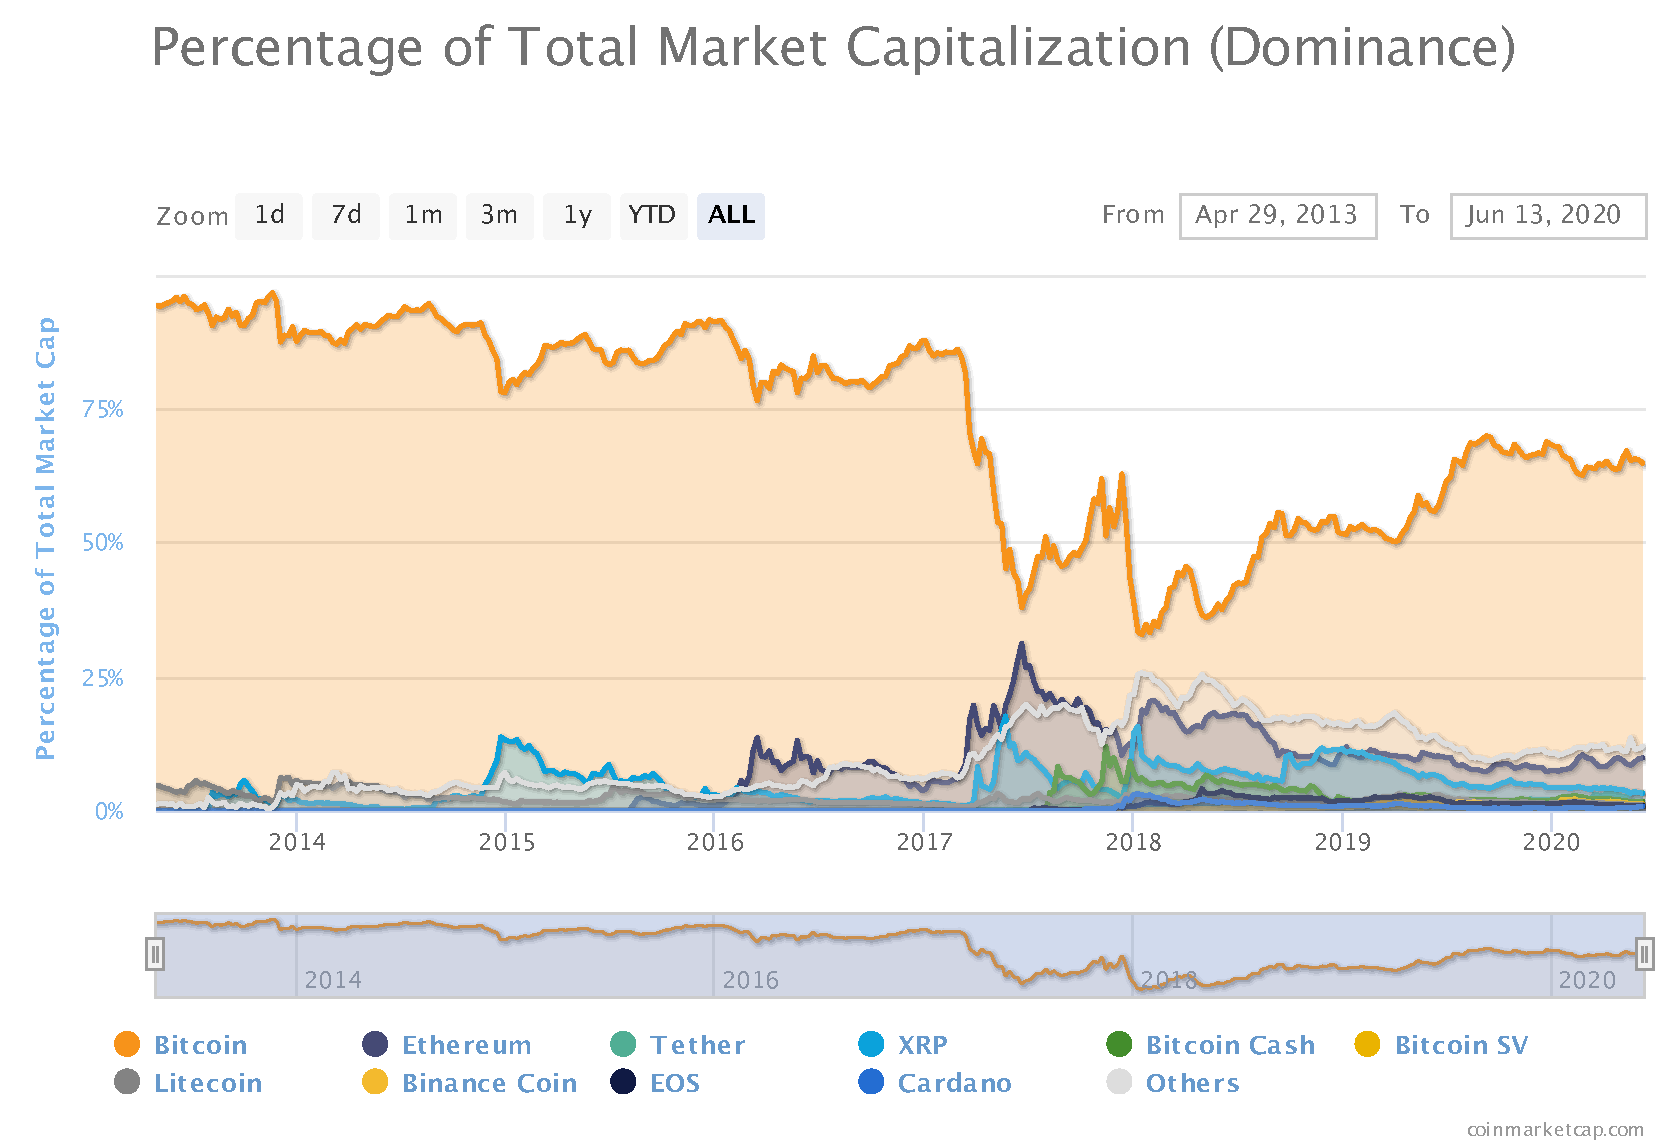
\includegraphics[width=\textwidth,draft=False]{figures/percentage-of-total-mark.pdf}
    \caption[Market Dominance]{Source: \citep{coinmarketcap}.}
    \label{fig:dominance}
\end{figure*}

\section*{Introduction}
This paper originated from my seminar work in the summer semester 2020 at the University of Applied Sciences Wedel, which was supervised by \textsc{Prof. Dr. Beuster}. This paper is about cryptocurrencies and the different aspects under which these can be assessed. It is based on the same-titled paper by \citet{Feder2018TheRA}.  

There exist at the time of this writing 5,576 different, traded cryptocurrencies. However, all of them were created after the rise of Bitcoin, which was invented in 2009. Cryptocurrencies themselves have been around since the early '80s, yet they gained true success only in the last decade. While Bitcoin is the most traded cryptocurrency today, many new coins have also emerged with varying levels of success. Recent developments, like the Bitcoin bubble in 2017 indicate a shift in the markets. Bitcoins' total leadership in the industry seems to have faded off, having only a mere market dominance of 64,7\%, resulting in other currencies growing stronger, like Ethereum or Tether. While the number of 5,576 cryptocurrencies may seem big, this is only the amount of coins that made it to the exchanges. Research shows that 85\% of all announced coins fail even before reaching the market. Furthermore, 44\% of all publicly traded coins have been abandoned at some point in time, with 18\% of them even forever \citep{Feder2018TheRA}. 

This paper is divided into three different segments: The first part focuses on the background of cryptocurrencies and gives an overview of the field. The next part describes the ongoing research of market dynamics. Lastly, in the third part, I will discuss the rise and fall of cryptocurrencies. This paper aims to give an overview of the current state of the cryptocurrency field and its past.
\tableofcontents
\pagebreak


\section{Background}\label{background}

When two people want to exchange money on the internet, they typically need a trusted third party, like PayPal or a bank, as otherwise, the risk of getting ripped off is too high. In many cases, these middlemen take a percentage of the exchanged money as a transaction fee. In addition, the transaction is susceptible to fraudulent behavior and a small percentage of fraudulent transactions is accepted as unavoidable.

Cryptocurrencies aim to solve this problem, as they offer the ability to exchange money directly. They base on the idea of a cryptographic proof instead of trust and thus allowing any two strangers to exchange money safely without a middleman. As transactions in cryptocurrencies are computationally impractical to reverse, they further protect against fraud. The transactions are often recorded in a public distributed ledger, which protects against the double-spending problem in peer-to-peer networks \cite{Bitcoin}. 

The idea of this is certainly not new: \textit{ecash} was proposed in 1983 and was the first cryptocurrency \cite{ecash1, ecash2}. In 1989 it was implemented by \textit{Digicash} and allowed for anonymous, untraceable payments. As it failed to get enough merchants to accept the currency, it had to shut down in 1998 and sold off its assets \cite{digicash}.

A few other concepts emerged later on, like one described in a paper from the NSA \cite{nsa} or \textit{b-money} \cite{bmoney}. Like before, they also did not really catch on. This however changed in 2009: \textit{Bitcoin} was announced and improved on the ideas of previously failed currencies \cite{Bitcoin}. While it took a few years to really gain traction, it is now the top one cryptocurrency and turned the field into an industry, with a market capitalization of \$268 billion, and an all-time peak of \$830 billion.




\autoref{fig:dominance} shows the percentage of the market capitalization with respect to the currency from 2013 to 2020. It can be seen that in the first years' Bitcoin dominated the market by a large margin. When mid-2017 arrived, things changed: Bitcoin lost a large amount of market capitalization, and newer cryptocurrencies, like Ethereum, grew. Additionally, it can be noted that the market share of ``Others" also increased. This is due to the ever-growing interest in cryptocurrencies, which sparked the creation of many new currencies. In many cases, these new coins were relatively moderate changes from already existing currencies and sometimes scams \citep{deadcoins}. It too set off the creation of websites that advertise with the phrase ``easiest way to launch a Coin in 10 minutes!" \citep{cryptonote, cryptolife}, leading to 5,576 different traded cryptocurrencies \citep{coinmarketcap}.

\subsection{Major Cryptocurrencies}
Today, only 17 currencies have a market capitalization of more than one billion U.S. Dollar. By far the biggest currency is Bitcoin with \$173 billion. Ethereum follows it with a market capitalization of \$26 billion. Tether, Litecoin, and Monero each have less than \$10 billion. Cryptocurrencies other than Bitcoins are often referred to as Altcoins, as they offer an alternative to Bitcoin.

\subsubsection{Bitcoin}

As already introduced in \autoref{background}, Bitcoin marked the beginning for the overwhelming growth in cryptocurrencies as we know it today. The market took off slowly, with a massive price peak in late 2013, with prices from around \$150  (mid-2013) to over \$1100  (1th December 2013). This however did not last long and led to a steady decline in prices, ending in early 2015 with a price back again at \$200.

\begin{figure}[H]
    \centering
    \includegraphics[width=\linewidth]{figures/Bitcoin-charts.pdf}
    \caption[Bitcoin Price Chart]{Bitcoin Price Chart. Source: \citep{coinmarketcap}. }
    \label{fig:Bitcoin}
\end{figure}

In 2017 the fall was over and Bitcoin started to rise again: By early 2017, Bitcoins value was again over \$1000  and at the end of 2017 the value rose to over \$19,000. This caused a massive sell-off and prices began to fall until the end of 2018 again. Since then is Bitcoin steadily rising and falling again.   

\subsubsection{Ethereum}
Ethereum is a cryptocurrency, which is not based on Bitcoin. It went live on July 30, 2015, and offers in addition to Bitcoin not only the possibilities of a payment network but also to run decentralized applications on its blockchain. This allows for smart contracts, which behave like a program that automatically executes when specific conditions are met. The use of the blockchain allows here for high availability and resistance against censorship, fraud, or any other third party interference. It is nowadays the second-largest cryptocurrency with a market capitalization of around 10\%.

\begin{figure}[H]
    \centering
    \includegraphics[width=\linewidth]{figures/Ethereum-charts.pdf}
    \caption[Ethereum Price Chart]{Ethereum Price Chart. Source: \citep{coinmarketcap}. }
    \label{fig:Ethereum}
\end{figure}

Its valuation is a lot more stable than for example Bitcoins: It had gained traction in early 2017 and rose, like Bitcoin, to an all-time high of \$1200  in early 2018. It can be noted, that while Ethereum did still fall in the long run, it was more stable than Bitcoin in the first month after Bitcoins massive selloffs: Where Bitcoin lost nearly 50\% of its value, Ethereum even gained value, having at the first of February 2018 a value of around \$1000. By the end of 2018, Ethereum stopped falling at a value of \$90  and started rising again, to at the moment around \$240.

\subsubsection{Tether}
Besides Bitcoin and Ethereum exists Tether, which is nowadays the third-largest cryptocurrency with a market capitalization of a little under \$10 billion. It launched in 2014 with the idea to mirror the U.S. Dollar. As it is ``tethered" (hence the name) to the U.S. Dollar, the Tether coin\footnote{A coin is synonym to the unit of currency.} is more stable than Bitcoin or Ethereum. In the beginning, Tether used Bitcoins transport protocol but later changed to an Ethereum Token. In total, Tether is issued on both Bitcoin and Ethereums, but also on EOS and Tron blockchains.

\begin{figure}[H]
    \centering
    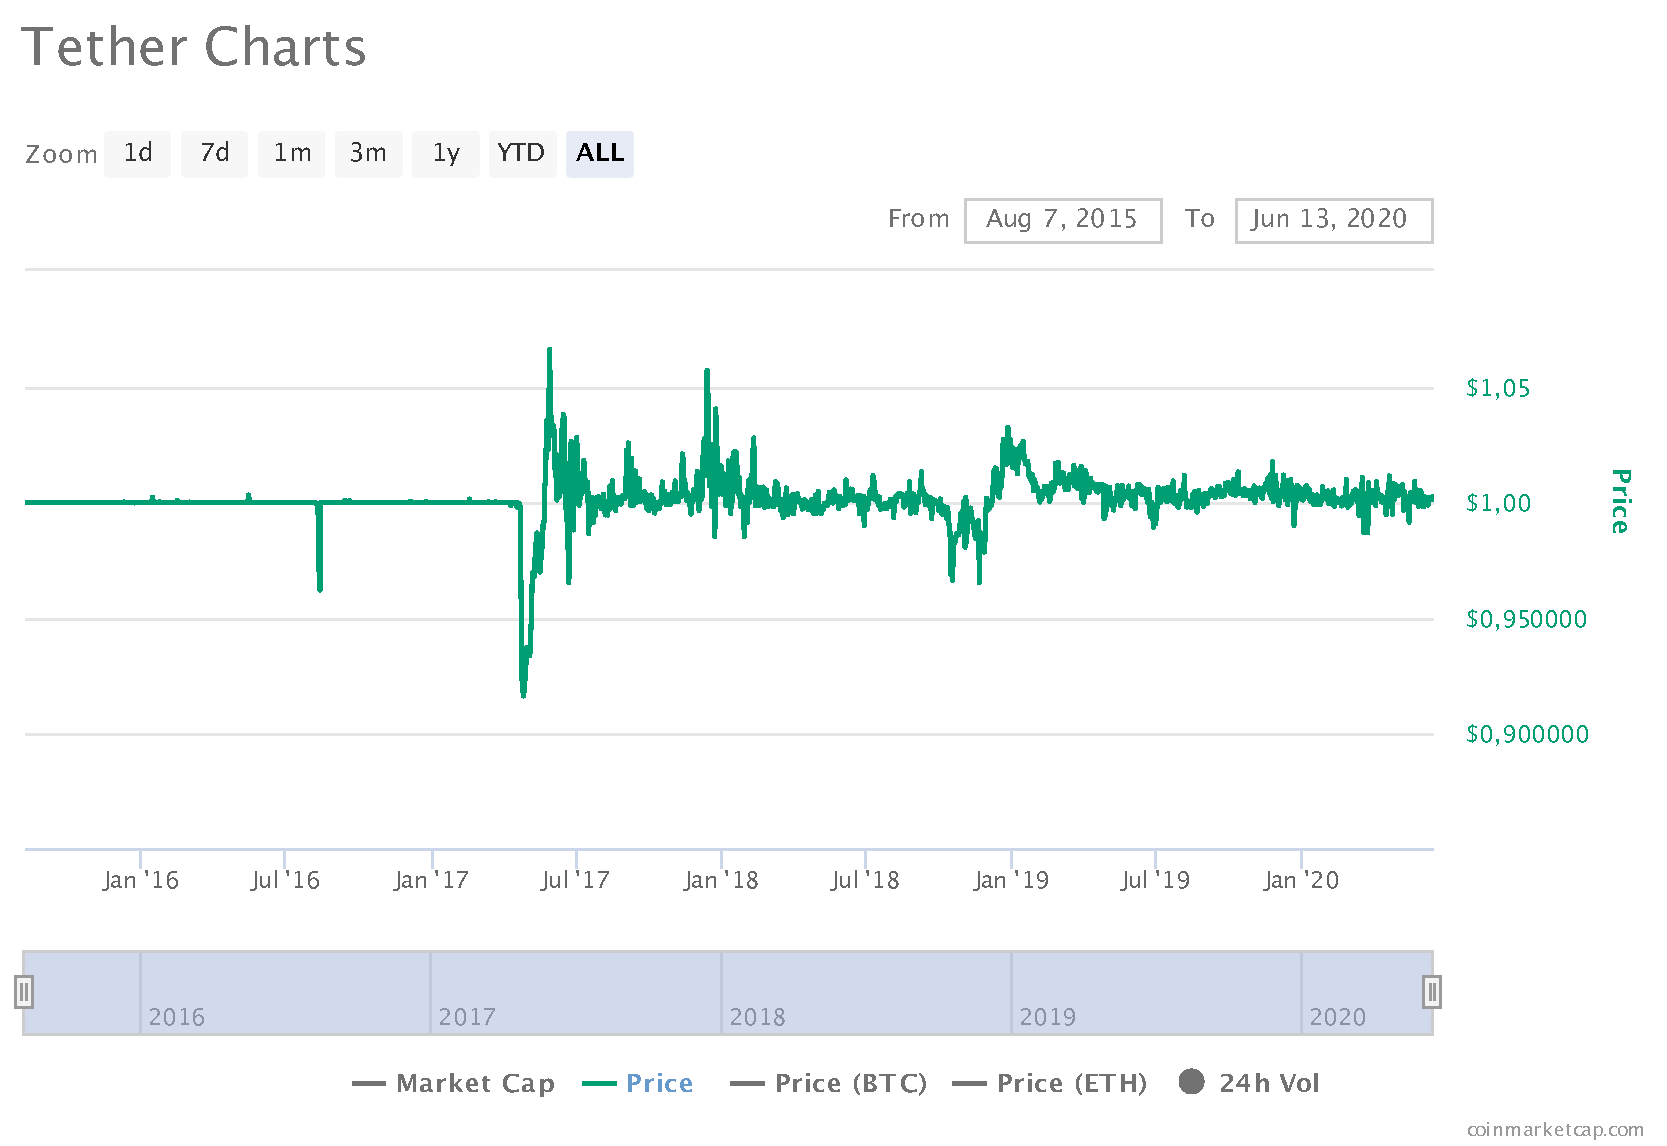
\includegraphics[width=\linewidth]{figures/tether-charts (1).pdf}
    \caption[Tether Price Chart]{Tether Price Chart. Source: \citep{coinmarketcap}. }
    \label{fig:Tether}
\end{figure}

\subsubsection{Litecoin}
The seventh-largest cryptocurrency with a market capitalization of a bit less than \$3 billion  today is Litecoin. Litecoin was one of the first coins after Bitcoin and launched in 2011. It is based on Bitcoins protocol but differs in a few factors like the hashing algorithm used and block transaction times. Litecoin aimed for a lot quicker confirmation speed, which is about 2.5 minutes per block, but may take up to 30 minutes when the network is congested. A quicker confirmation speed is helpful when the currency is aimed to be used for example in stores. The quicker the network confirms that the transaction has successfully happened, the faster the payment process can be. 

\begin{figure}[H]
    \centering
    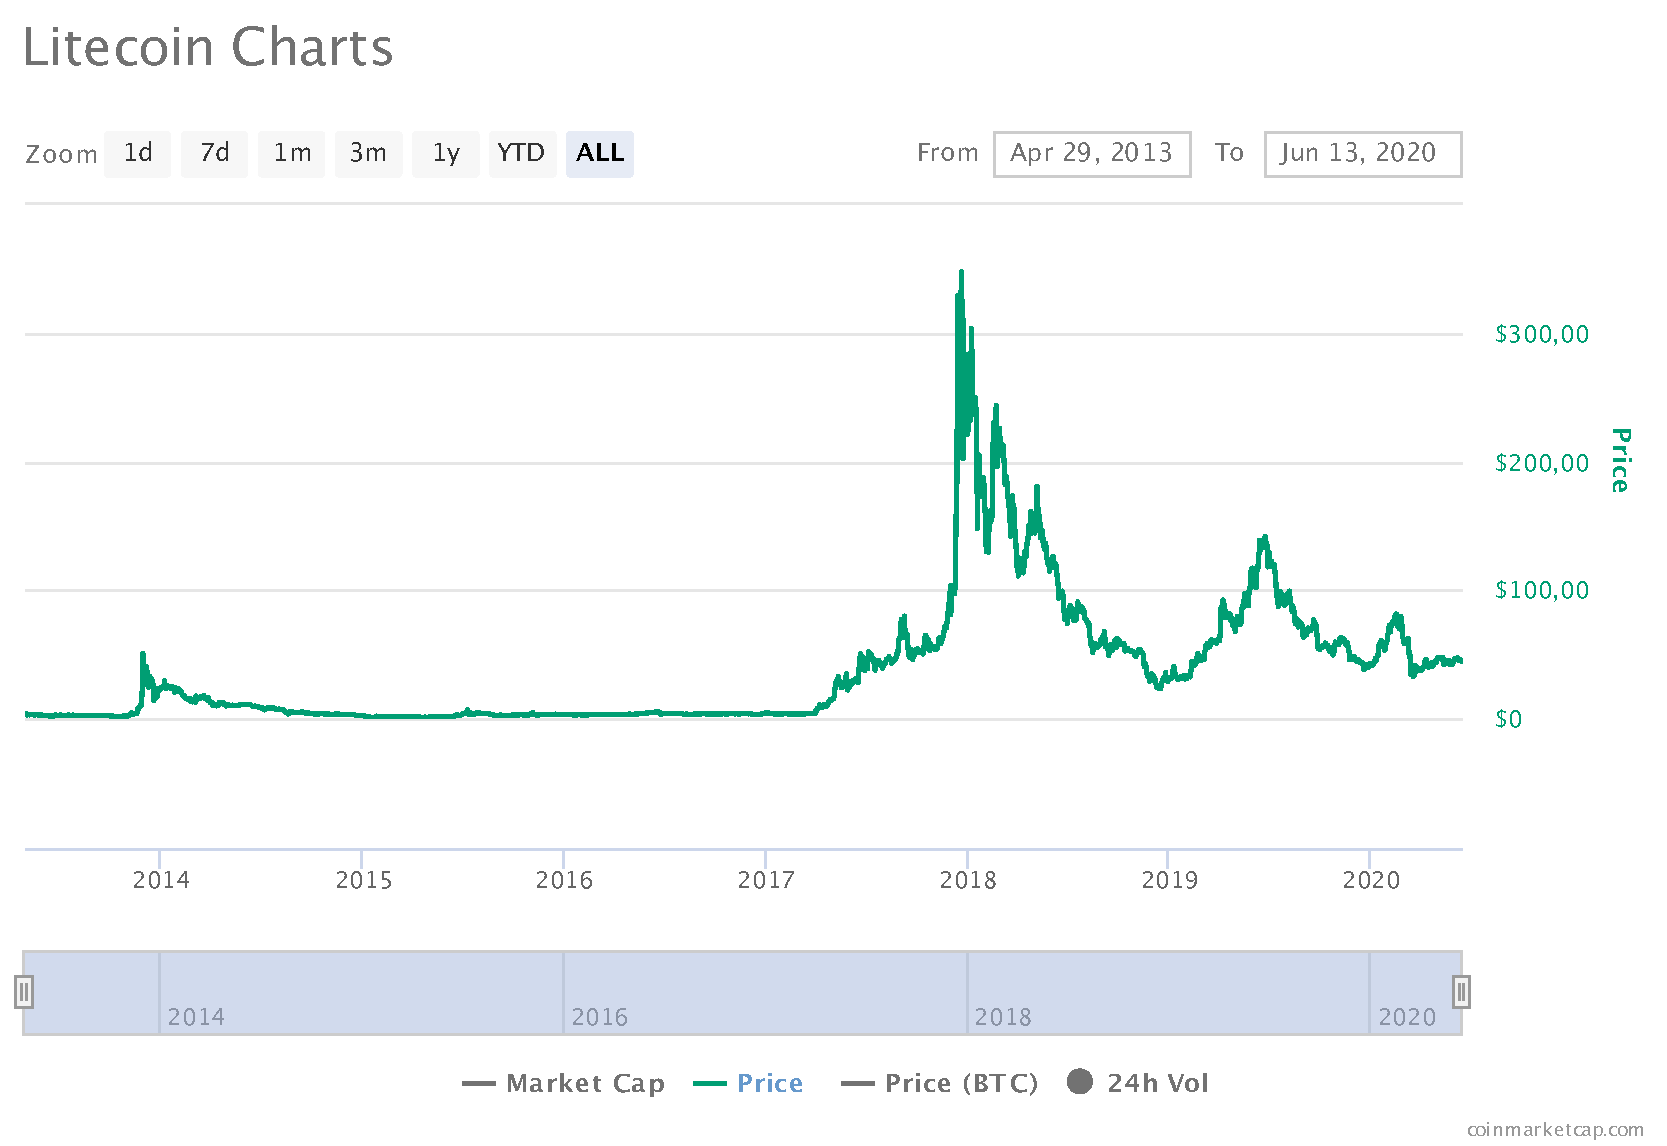
\includegraphics[width=\linewidth]{figures/litecoin-charts.pdf}
    \caption[Litecoin Price Chart]{Litecoin Price Chart. Source: \citep{coinmarketcap}. }
    \label{fig:Litecoin}
\end{figure}

As it was intended as a lite version of Bitcoin, the prices do rise and fall at roughly the same time. Litecoin however never reached the same highs as Bitcoin, having its all-time high at a little over \$375. 

\subsubsection{Monero}
Monero started as a privacy-oriented alternative. While Bitcoin movements can be traced using the blockchain, Moneros transactions are anonymous, hiding the balances of a certain wallet or transactions from further inspection. It is a fork of ByteCoin, with the addition of incorporating certain features, which make it resistant against custom-built ASICs for mining, resulting in a still profitable mining operation on modern CPUs and GPUs. These properties make Monero an ideal choice for criminals, as they do not need to launder their earnings like they would have to do with Bitcoin and the other currencies. The market capitalization is just above one billion U.S. Dollar.

\begin{figure}[H]
    \centering
    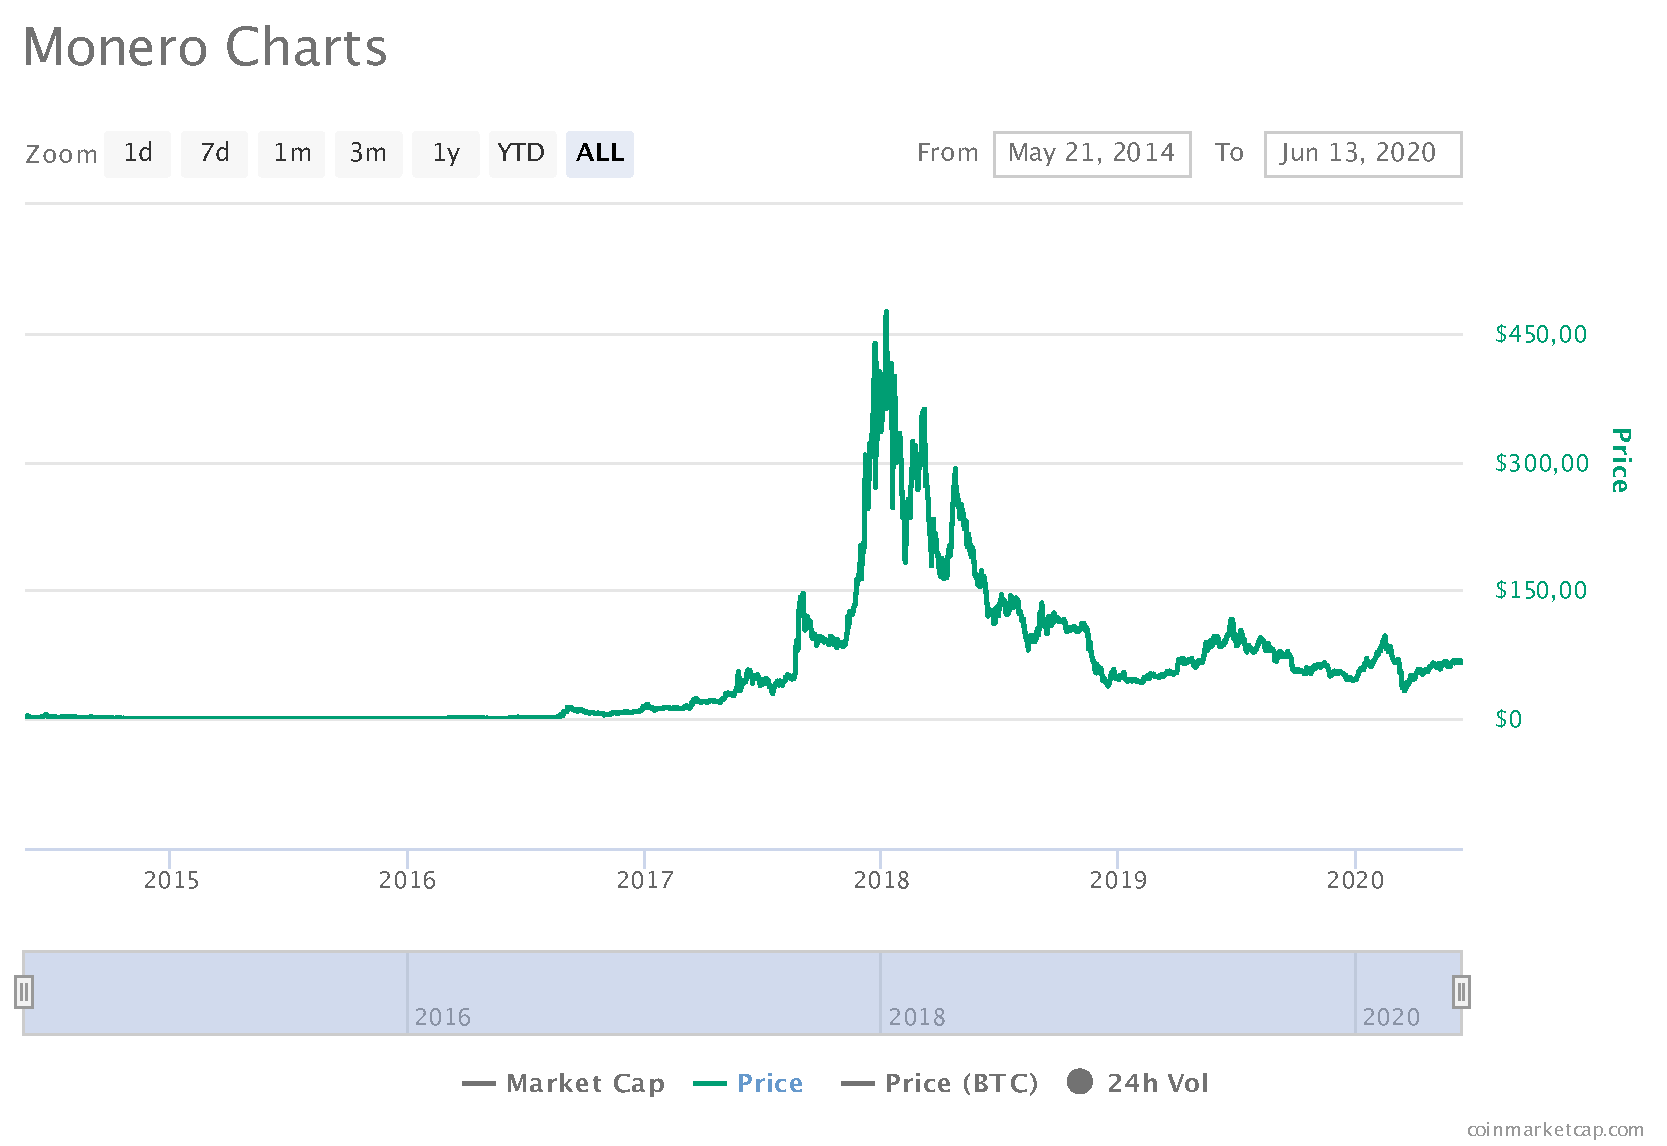
\includegraphics[width=\linewidth]{figures/monero-charts.pdf}
    \caption[Monero Price Chart]{Monero Price Chart. Source: \citep{coinmarketcap}. }
    \label{fig:Monero}
\end{figure}

Like the other currencies, except Tether, Monero rose with Bitcoins' rise and too fell with it.  However, unlike the others, Monero did not rise and fall as much anymore after 2018, but more or less stood steady at around \$60.  

\subsection{Cryptocurrency Markets} 
\begin{figure*}
    \centering
    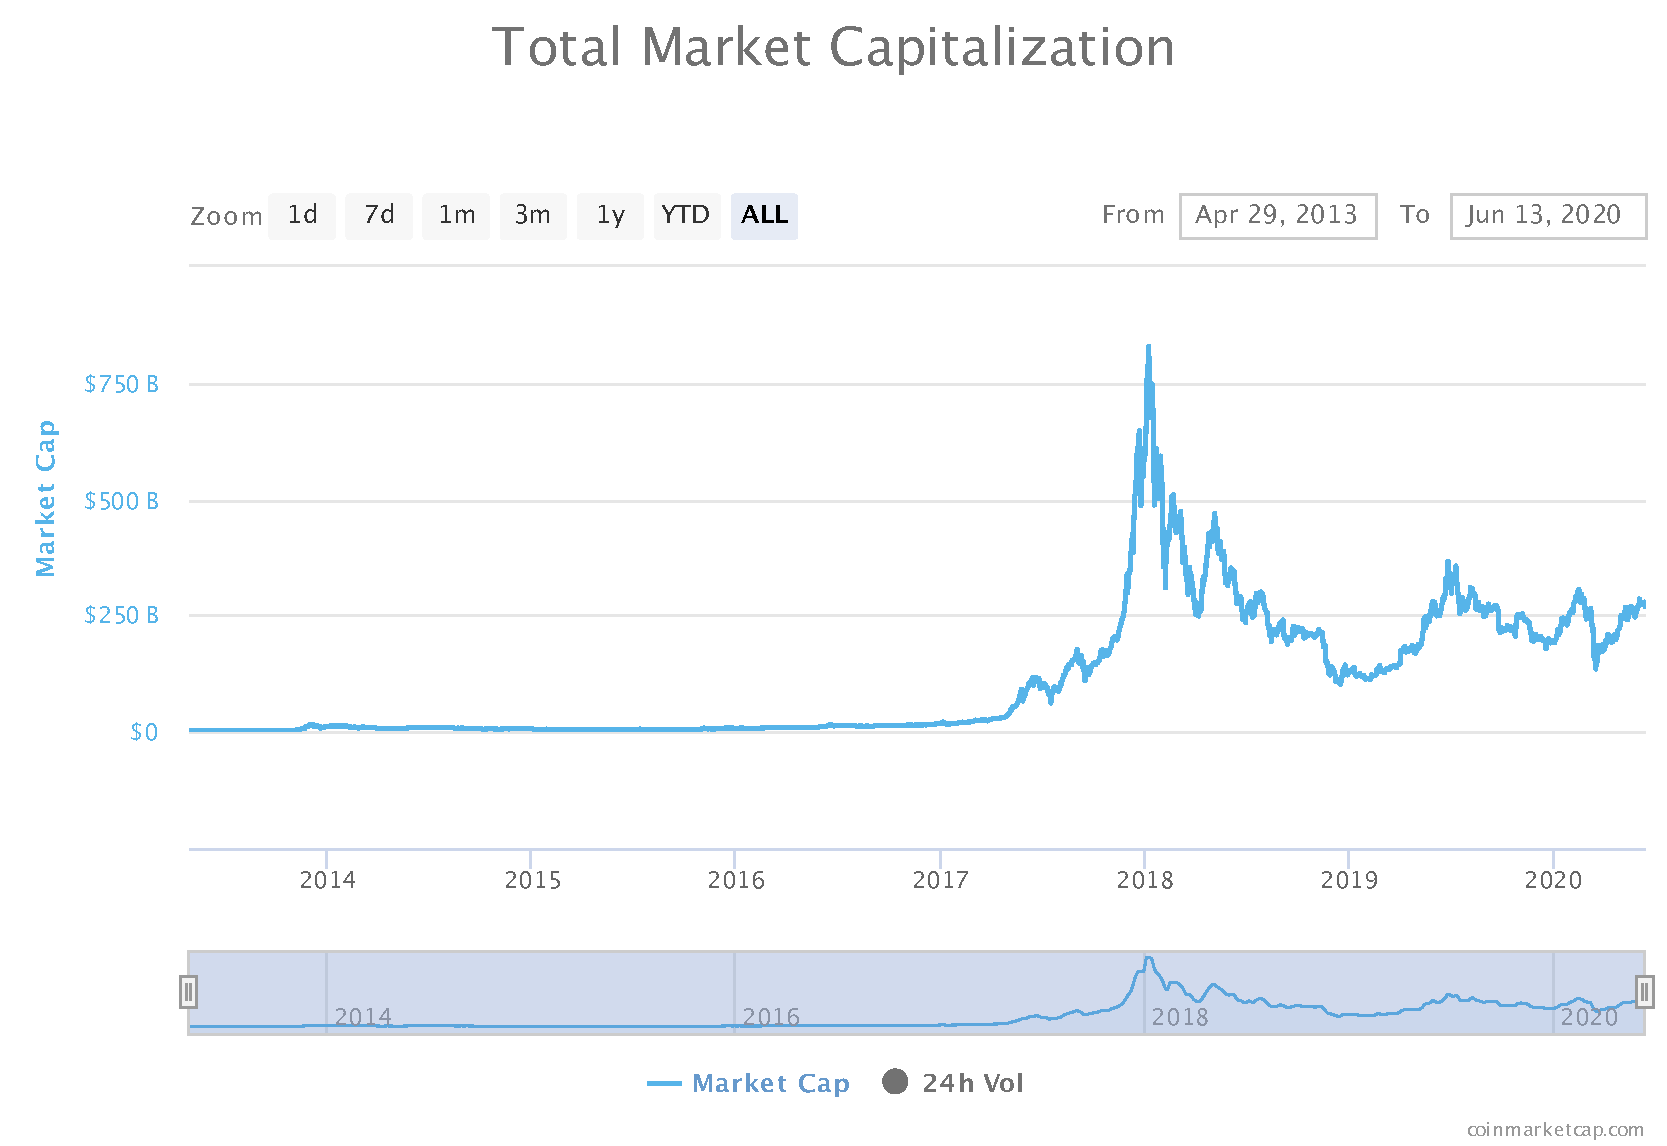
\includegraphics[width=\linewidth]{figures/total-market-capitalizat.pdf}
    \caption[Cryptocurrency Market Capitalization]{Source: \citep{coinmarketcap}. }
    \label{fig:total-cap}
\end{figure*}

Most of the prices are driven by demand and supply at exchanges. Similar to other exchanges, a person can go to an exchange and trade a currency for another one, like U.S. Dollars for Bitcoins or Bitcoins for Litecoins, as an example. As these exchanges are unregulated, they sometimes pose some form of risk. Famous examples are the exchange Mt.Gox, which was at the time the biggest processor with 70\% of all Bitcoin trades \citep{wsj} or BTC-E, which was later called WEX. 

While Mt.Gox got hacked and went bankrupt afterward, ultimately resulting in the loss of around 7\% of all Bitcoins available, the fate of BTC-E was different: in 2017 US authorities seized the domain and 38\% of all customer funds, as they suspected that the market was used to launder money from the Mt.Gox hack. This led to the creation of WEX, which promised to pay back any of the customers' funds, but later disappeared completely overnight \citep{wexnzcase}. 

These incidents however did not stop cryptocurrencies from growing into a more and more valuable market.  

\autoref{fig:total-cap} shows the total market capitalization of the cryptocurrency market. There can be seen the two major spikes compared to the time before and after: a more subtle one from 2013 to 2014, and a massive one from 2017 to 2018. The first bubble was likely to be due to price manipulation in the Bitcoin market \citep{article}, where prices began to rise in just two months from \$150  to over \$1000. After the bubble had burst, it triggered the first massive rise in new cryptocurrencies being announced, as it can be seen in \autoref{fig:announcedvstraded}. 

\begin{figure}[ht]
    \centering
    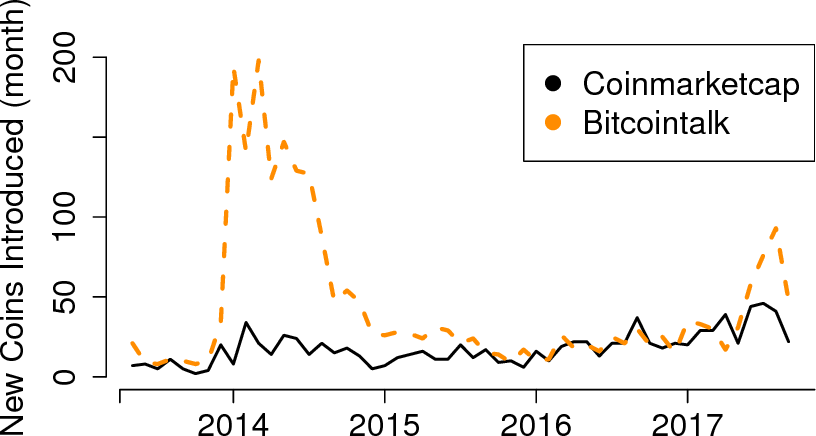
\includegraphics[width=\linewidth,  draft=false]{figures/13-Figure6-1.png}
    \caption[Announced currencies vs traded]{New cryptocurrencies announced compared to new currencies traded. Source: \citep{Feder2018TheRA}.}
    \label{fig:announcedvstraded}
\end{figure}

What else can be seen is, that most of the announced coins never reached the market. Research has shown that before the spike in 2013, there were mostly no network effects\footnote{The more popular a cryptocurrency is, the more it will become adopted and thus useful, resulting in more participants in the market.} or winner-take-all\footnote{Development towards only one currency} dynamics \citep{predictwinner}. With the market flooded with newly announced coins, this changed. As more and more currencies reached the exchanges, their values started to decline, while Bitcoin's started to slowly rise again. This can also very well be seen in \autoref{fig:dominance}, where Bitcoins share only very gently declined, while the other coins had a hard time to gain market value.  

The second peak in late 2017 once again reversed the situation: When Bitcoin started to depreciate again, other cryptocurrencies, which came later to the market, like Ripple or Ethereum, still continued to rise. This indicates a move away again from the clear winner-take-all effect. 

\section{Market dynamics of Cryptocurrencies}
The paper from \citet{Feder2018TheRA} studied the trading activity associated with 1082 currencies in the time period of 2013 to 2018. In their research, they show that only a few of the many announced coins make it to the markets. But that does not mean success, as they show that these coins also have a high chance that they become abandoned.

\subsection{Classification of the state of a coin}
To determine whether or not a coin is still used, they identified peaks in trading volume on the different markets. They define a peak as \textit{``a day in which the 7-day rolling average value is greater than any value 30 days before or after"}, which also has to satisfy two additional criteria:
\begin{itemize}
    \item The peak is greater or equal to 50\% of the minimum value in the last 30 days and
    \item must be at least 5\% as large as the maximum peak
\end{itemize}

From these peaks, they define if a cryptocurrency is abandoned. By comparing the peak values to the following days' trading volume values, they can determine its state. If the volume for a month is less than or equal to 1\% of the peak volume, it is considered abandoned and no longer used.

This does not necessarily mean that the currency will never be used, as this is unlike other markets not a ``one-way road". When trading of the currency picks up again, the coin is resurrected. 

\begin{figure}[ht]
    \centering
    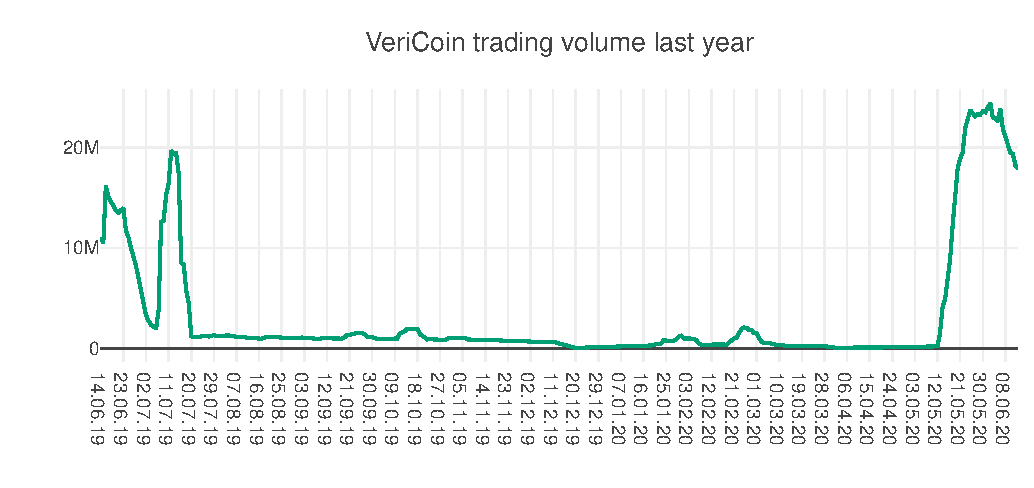
\includegraphics[width=\linewidth]{figures/diagram-20200614.pdf}
    \caption[Trading volume of VeriCoin]{7 day rolling average over the trading volume of VeriCoin for the last year.}
    \label{fig:tradingvolvericoin}
\end{figure}


One example of such behavior can be found in the currency VeriCoin. \autoref{fig:tradingvolvericoin} shows the trading volume over a year. We can see, that in mid-2019 the currency still was still traded slightly with an average volume just shy of 20 million, but was abandoned for much of the rest of 2019 and most of 2020. Only very recently it got resurrected and got traded again at slightly higher volumes. 

\begin{figure}[ht]
    \centering
    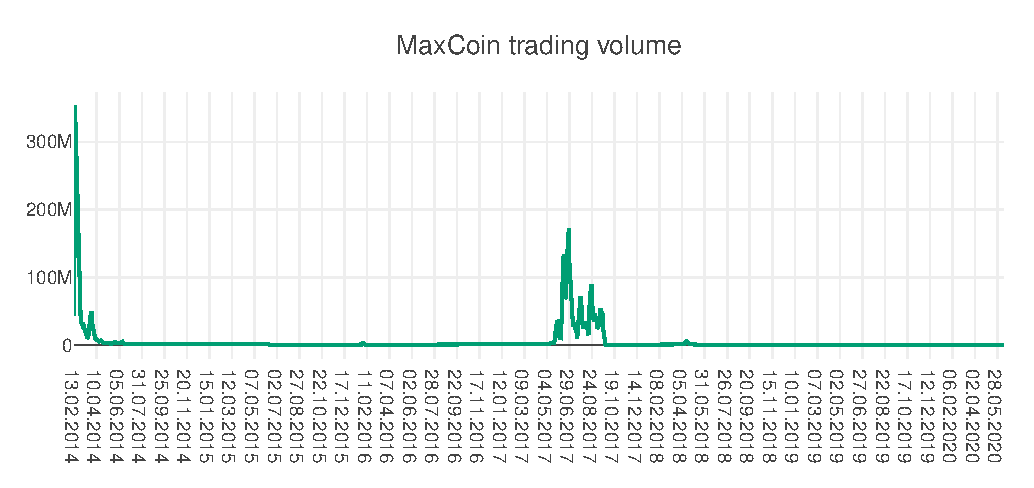
\includegraphics[width=\linewidth]{figures/diagram-20200614 (3).pdf}
    \caption[Trading Volume of MaxCoin]{7 day rolling average over the trading volume of MaxCoin.}
    \label{fig:tradingvolmaxcoin}
\end{figure}

A more permanent fate seems to have happened to MaxCoin: While it started with a high trading volume of 300 million in 2014, it quickly dropped and became abandoned. It was later resurrected in 2017 but seems to have now been permanently abandoned again, as the trading volume never rose again and is sometimes even as low as zero.

\subsection{Results of peak analysis}
\begin{table*}
\centering
\resizebox{\textwidth}{!}{%
\begin{tabular}{@{}lcccccc@{}}

                                                      & overall                   & \textless{}\$1M  & \$1--10M  & \$10--100M & \$100M--1B & \textgreater{}\$1B \\ \toprule
\multicolumn{1}{l|}{\# coins}                         & \multicolumn{1}{c|}{1082} & 374                 & 344         & 183       & 124       & 57                 \\ \midrule
\multicolumn{1}{l|}{\# total price peaks}             & \multicolumn{1}{c|}{3508} & 1426                & 1022        & 531       & 376       & 153                \\ \midrule
\multicolumn{1}{l|}{\# total volume peaks}            & \multicolumn{1}{c|}{3828} & 1734                & 1064        & 468       & 406       & 156                \\ \midrule
\multicolumn{1}{l|}{\# abandonments}                  & \multicolumn{1}{c|}{642}  & 347                 & 192         & 62        & 41        & 0                  \\ \midrule
\multicolumn{1}{l|}{\# median days abandoned}         & \multicolumn{1}{c|}{182}  & 153                 & 184         & 242       & 426       & ---                \\ \midrule
\multicolumn{1}{l|}{\# resurrections}                 & \multicolumn{1}{c|}{336}  & 183                 & 103         & 25        & 25        & ---                \\ \midrule
\multicolumn{1}{l|}{\# median months to resurrection} & \multicolumn{1}{c|}{6}    & 5                   & 6           & 10        & 19        & ---                \\ \midrule
\multicolumn{1}{l|}{\# coins permanently abandoned} & \multicolumn{1}{c|}{190}                       & 86                  & 57          & 32        & 15        & 0                  \\ \bottomrule \\
\end{tabular}%
}

\caption{Summary statistics Source: \citep{Feder2018TheRA}. Categorized by total trading volume per coin.}
\label{tab:my-table}
\end{table*}
As a result of this analysis, it showed that from the 1,082 currencies, 1,068 had at least one price and volume peak. In total, they found 3,508 price peaks and 3,828 volume peaks. \autoref{tab:my-table} shows a short version of their findings.

Although these values are somewhat dated now, as they are from 2018 and, for example, the amount of abandoned coins has risen nowadays to 1928 \citep{deadcoins}, they still show a clear trend. 

From the table It is clear that most coins do not attract a large number of trades. Over 65\% of all analyzed coins have traded in their total lifespan, at that time, less than \$10 million. While they are the reason for the most price and volume peaks, the number of peaks per currency has a median of just three, regardless of the trading volume. 

Moreover, it shows that the less traded coins have a higher risk to get abandoned at some point, and sometimes even forever. While higher volume coins tend to get less abandoned, they also tend to get abandoned longer than less traded coins and take longer to get resurrected, if they even do so---the table shows that if a large volume currency is getting abandoned, then its chance to get resurrected is lower than a lower volume one.

Furthermore, they find that what matters the most is the median time and the median increase in trade volume to the first peak. The reasoning is that the first peaks are defined by the early backers, who stand behind a currency before the general public does. 

\begin{table}[h]
\centering
\resizebox{\linewidth}{!}{%
\begin{tabular}{@{}l|c|c|c@{}}

                                & overall & \textless{}\$1M  & \textgreater{}\$1B \\ \toprule
median increase in trade volume & 3714\%  & 917\%               & 90530\%            \\ \midrule
median increase in price        & 749\%   & 418\%               & 3441\%             \\ \bottomrule  \\
\end{tabular}%
}

\caption{Median increases from launch to the first peak}
\label{tab:my-table2}
\end{table}
\autoref{tab:my-table2} shows that smaller currencies perform worse than the bigger ones. It should be noted of course, that bigger currencies are also more likely to experience bigger jumps.  

The other findings can be summarized as follows. Peaks after the initial tend to have a lower price rise, namely 200\% to 300\%. The highest price rises are found in the category of \$1--10 million trade volume, and the lowest in the category with \$100M--1B. 

When looking at the time period after the fall, it becomes apparent that lower value currencies fall farther, with 9 out of 10 currencies losing at least 40--50\%. Every second falls around 60--75\% and one in 10 even up to 80\%. Smaller cryptocurrencies are also exposed to higher median volume jumps: While often traded coins gain around 1500\% in volume increase around peaks, currencies with a trading volume of less than \$1 million  show numbers about the factor of 100 higher. However, it should also be noted that in 30\% of the time, these low volume currencies have days with zero tradings. The decrease in volume after the peak is consistent for all but the biggest currencies: it is common that the volume falls more than 90\% in the following month.

\subsection{Relationships between Key Variables}
\begin{figure*}
    \centering
    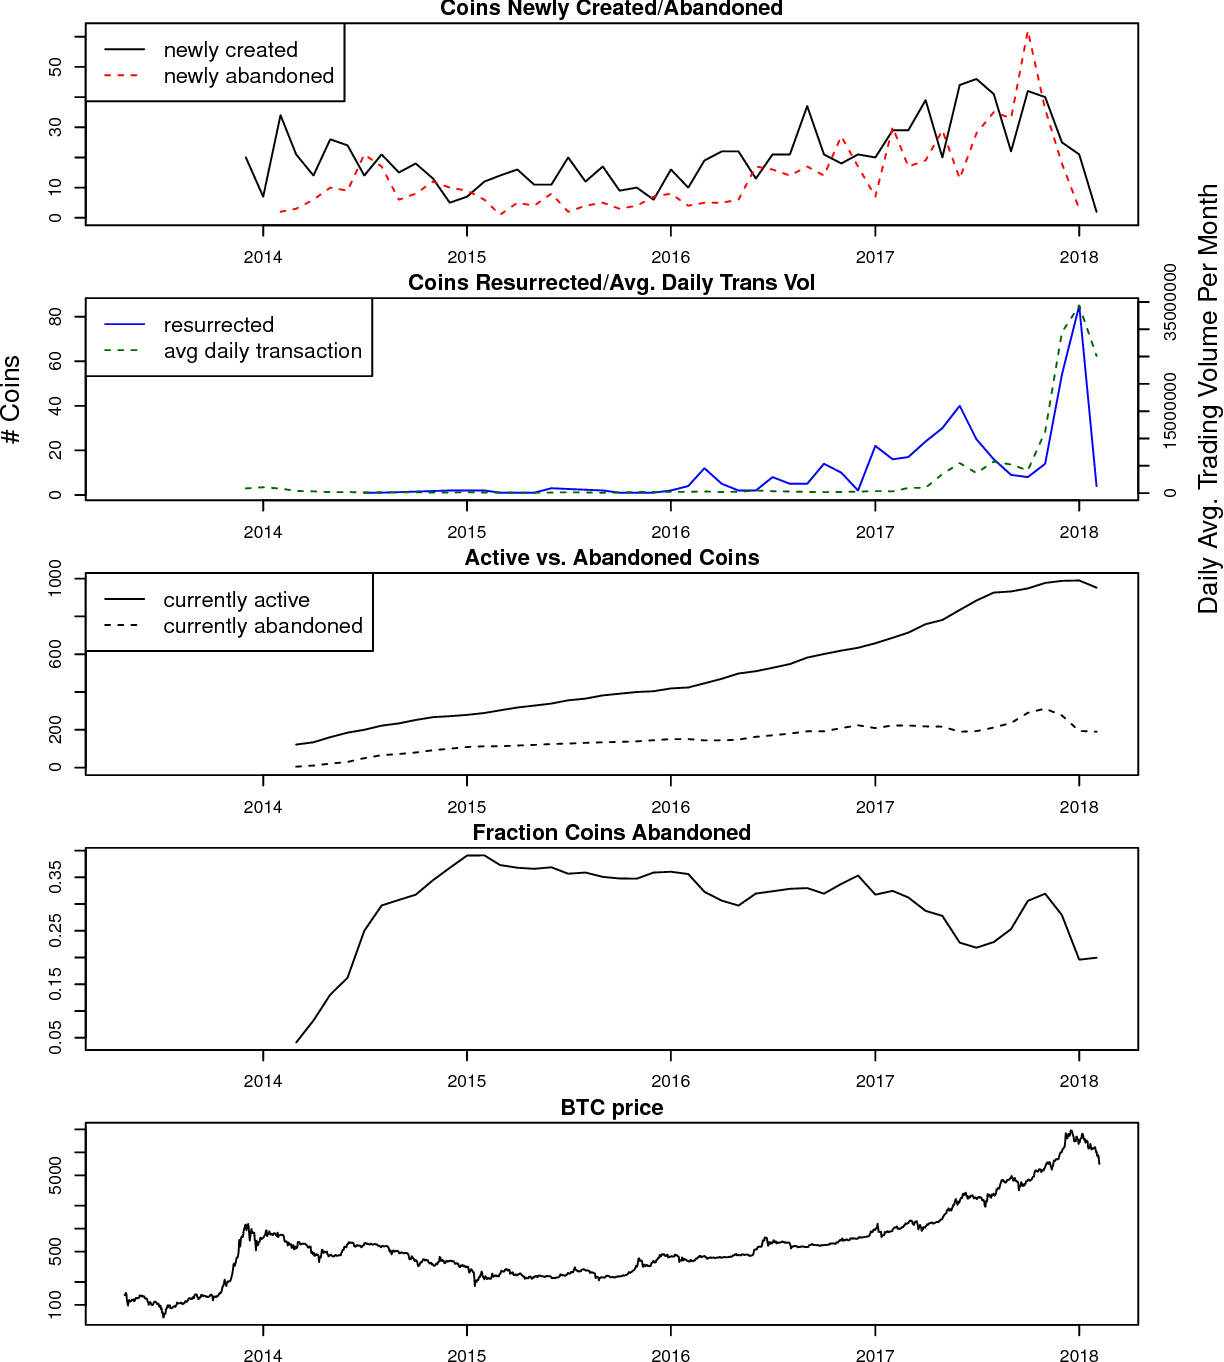
\includegraphics[width=.9\linewidth,  draft=false]{figures/16-Figure9-1.png}
    \caption[Summary of statistics]{Cryptocurrency summary statistics including abandonment, resurrection, creation, and daily average trading volume. Source: \citep{Feder2018TheRA}. }
    \label{fig:relations}
\end{figure*}

As it can be seen in \autoref{fig:total-cap} and the price charts in the first section (\autoref{fig:Bitcoin}, \autoref{fig:Ethereum}, \autoref{fig:Litecoin}, \autoref{fig:Monero}) there seems to be some kind of correlation between the price of Bitcoin and general interest in cryptocurrencies. It makes sense, that when Bitcoin is rising, one might invest into a previously created and maybe abandoned coin, hoping that it will rise the same way a little later, thus allowing the person to profit from extreme price rises. 

But not only old coins gain new interest, but new currencies are also created (again, \autoref{fig:total-cap} and \autoref{fig:dominance}), with some improving on the flaws of others (such as Ethereum) and some simply wanting to ``ride the wave". 

\begin{table*}
\centering
\resizebox{\textwidth}{!}{%
\begin{tabular}{p{2cm}ccccccc@{}}
\toprule
                               & \multicolumn{1}{p{1.5cm}}{\# Coins abandoned} & \multicolumn{1}{p{1.5cm}}{\# Coins resurrected} & \multicolumn{1}{p{1.5cm}}{\# Coins created} & \multicolumn{1}{p{1.5cm}}{Trade Volume} & \multicolumn{1}{p{1.5cm}}{Avg Bitcoin Price)} & \multicolumn{1}{p{1.5cm}}{\# Price Peaks} & \multicolumn{1}{p{1.5cm}}{\# Volume Peaks} \\ \toprule
\# Coins abandoned             & 1                                      &                                          &                                      &                                  &                                                    &                                    &                                     \\
\# Coins resurrected           & 0.2080                                 & 1                                        &                                      &                                  &                                                    &                                    &                                     \\
\# Coins created               & 0.6107                                 & 0.3858                                   & 1                                    &                                  &                                                    &                                    &                                     \\
Trade Volume                   & 0.0695                                 & 0.7512                                   & 0.0959                               & 1                                &                                                    &                                    &                                     \\
Average Bitcoin Price & 0.5321                                 & 0.7078                                   & 0.5053                               & 0.7996                           & 1                                                  &                                    &                                     \\
\# Price Peaks                 & 0.2756                                 & 0.8504                                   & 0.4515                               & 0.6524                           & 0.6798                                             & 1                                  &                                     \\
\# Volume Peaks                & 0.3795                                 & 0.9007                                   & 0.5013                               & 0.7072                           & 0.7756                                             & 0.9721                             & 1                                   \\ \bottomrule
\end{tabular}%
}
\caption{Monthly correlations between key variables in the ecosystem. Note that the average Bitcoin price is logarithmic. Source: \citep{Feder2018TheRA} }
\label{tab:my-table3}
\end{table*}

As by economic nature, one suspects that in times with massive price rises, the competition in a field will get stronger, whereas when prices fall, interest also falls, and thus only the best will survive. \autoref{fig:relations} shows the relationships between abandonment, resurrection, creation, and daily average trading volume. The first graph plots the newly created currencies against the abandoned ones on a monthly basis. When interest rose in early 2014, many new coins were introduced. But as Bitcoin crashed, it also led to less newly created and a rise in abandonment. After this the rates stabilized until 2016, where they started to rise, leading to a massive increase in late 2017. 

The next graph takes a look at resurrections versus the average daily transaction volume. It is apparent that they strongly correlate. The third and the fourth graph show that the amount of actively traded currencies rises more than the amount of currently abandoned currencies, with a trend to fewer abandonments overall. While in early 2015 over 35\% of all coins had been abandoned, this number fell to about 20\%. 

Note that the last graph is logarithmic. It plots the Bitcoin value in U.S. Dollar and makes it apparent that spikes in the graphs before, coincide with peaks in Bitcoins price, showing again Bitcoins' leadership in the cryptocurrency market.

\autoref{tab:my-table3} shows the correlations which have been found by \citet{Feder2018TheRA}. It shows that the resurrection of a coin is strongly tied to the number of the price (0.85) and volume (0.90) peaks, supporting the argument that many coins simply ``want to ride the wave".  

Digging deeper, one can find a positive correlation between the number of coins created and coins abandoned. This can be explained by the simple creation of more new coins after the abandonment of one. In many cases, these new coins then build upon the old coin, improving on its original weaknesses\footnote{One such example would be NXT. Created in 2013, abandoned not much later, yet it was used as the foundation of 11 new currencies\citep{mapofcoins}. }. Furthermore, this indicates some kind of competition between the coins, as other currencies get abandoned in favor of new and supposedly better ones. This however does not always have to be the case, as it can be seen by Bitcoin Gold\footnote{Bitcoin Gold is a hard-fork from Bitcoin and changed the hashing algorithm used to one, which is resilient against ASICs, favoring GPUs and thus `` democratizing" Bitcoin. It suffered a few attacks and is mostly dead now. }.

Lastly, when looking at the average Bitcoin price in correlation to the other variables, it becomes very clear that Bitcoin is still the leader in this ecosystem. Bitcoins' high correlations with a low of 0.50 and a high of 0.79 through all key variables, shows how much Bitcoin dominates this field and thus sets the trend for all other cryptocurrencies. With the rise of Bitcoin, many new currencies were created and with its fall many too fell. 

\subsection{Bursting of bubbles and their effects}
This aspect is also of further interest by \citet{Feder2018TheRA}, but it has also been of interest prior. \citet{article} showed that the first Bitcoin bubble in 2014 was likely due to price manipulation, but also showed in \citep{predictwinner} that when Bitcoin prices fell, the other currencies were also hugely impacted. 

\begin{figure}[ht]
    \centering
    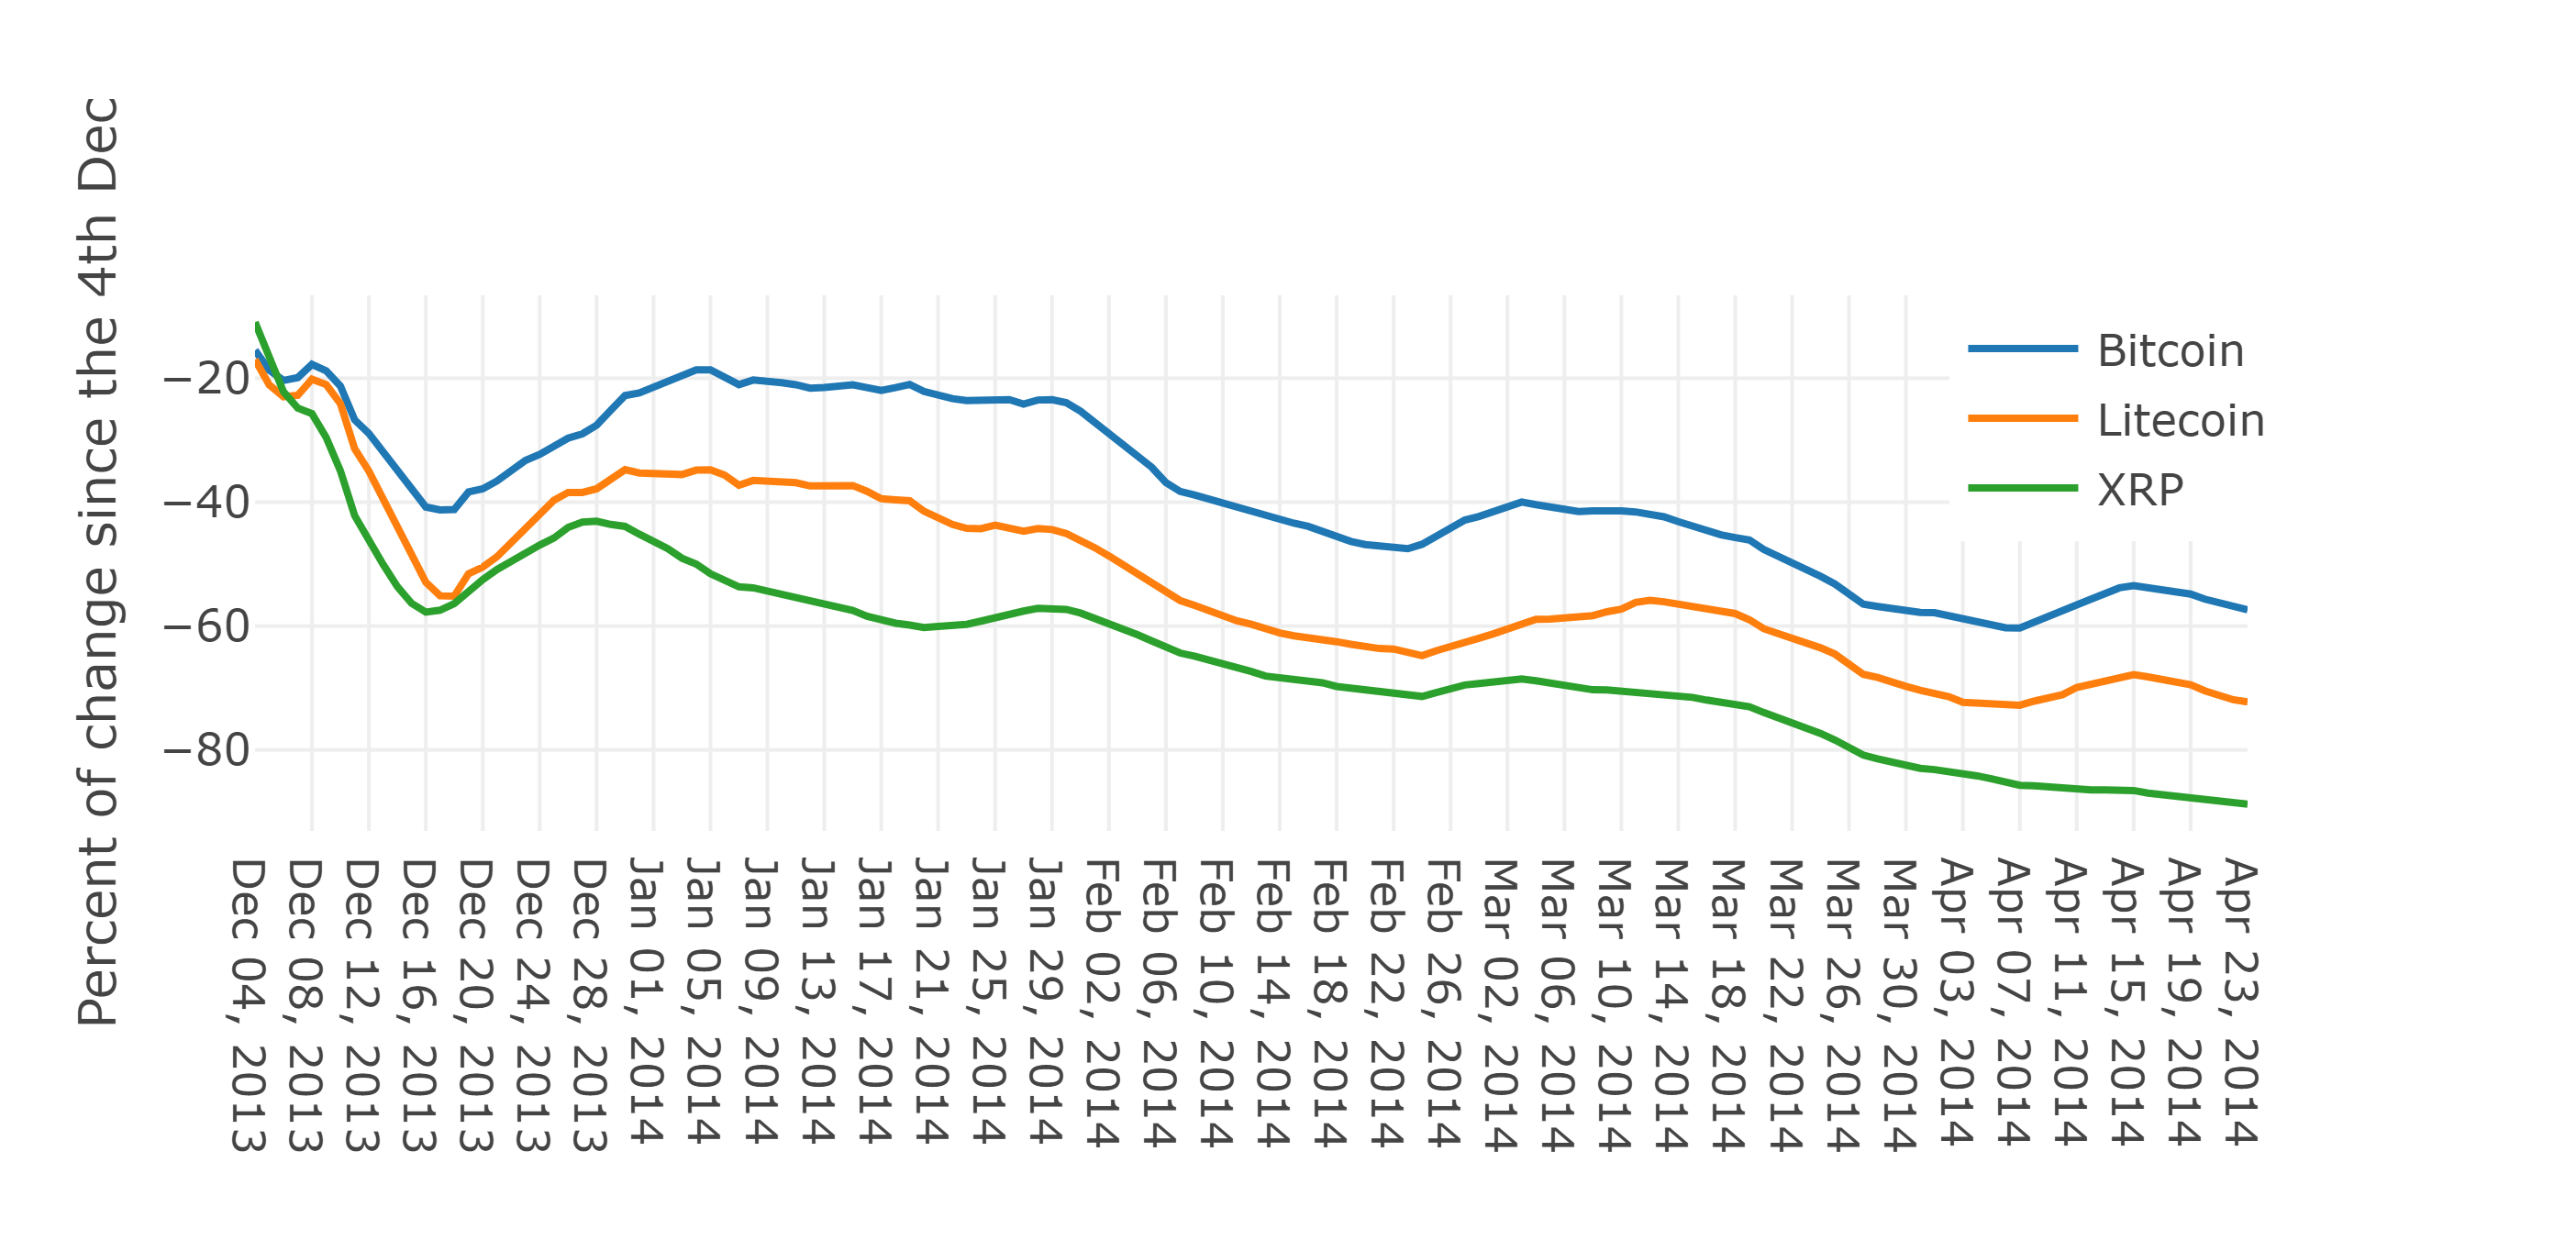
\includegraphics[width=\linewidth]{figures/diagram-20200618.png}
    \caption[Change in value after the 2013 Bubble]{7 day rolling average over change in percent in comparison to the 4th of December 2013.}
    \label{fig:bubble2013}
\end{figure}

\autoref{fig:bubble2013} plots the change in the value of the three biggest currencies at the time: Bitcoin, with around 90\% market share, Litecoin with nearly 5\%, and XRP, which was only created very recently, with 1.5\%. While Bitcoins fall was steep, with a decline of 60\%, others fell further: Litecoin fell by around 75\%, XRP even 88\%.

\begin{figure*}
    \centering
    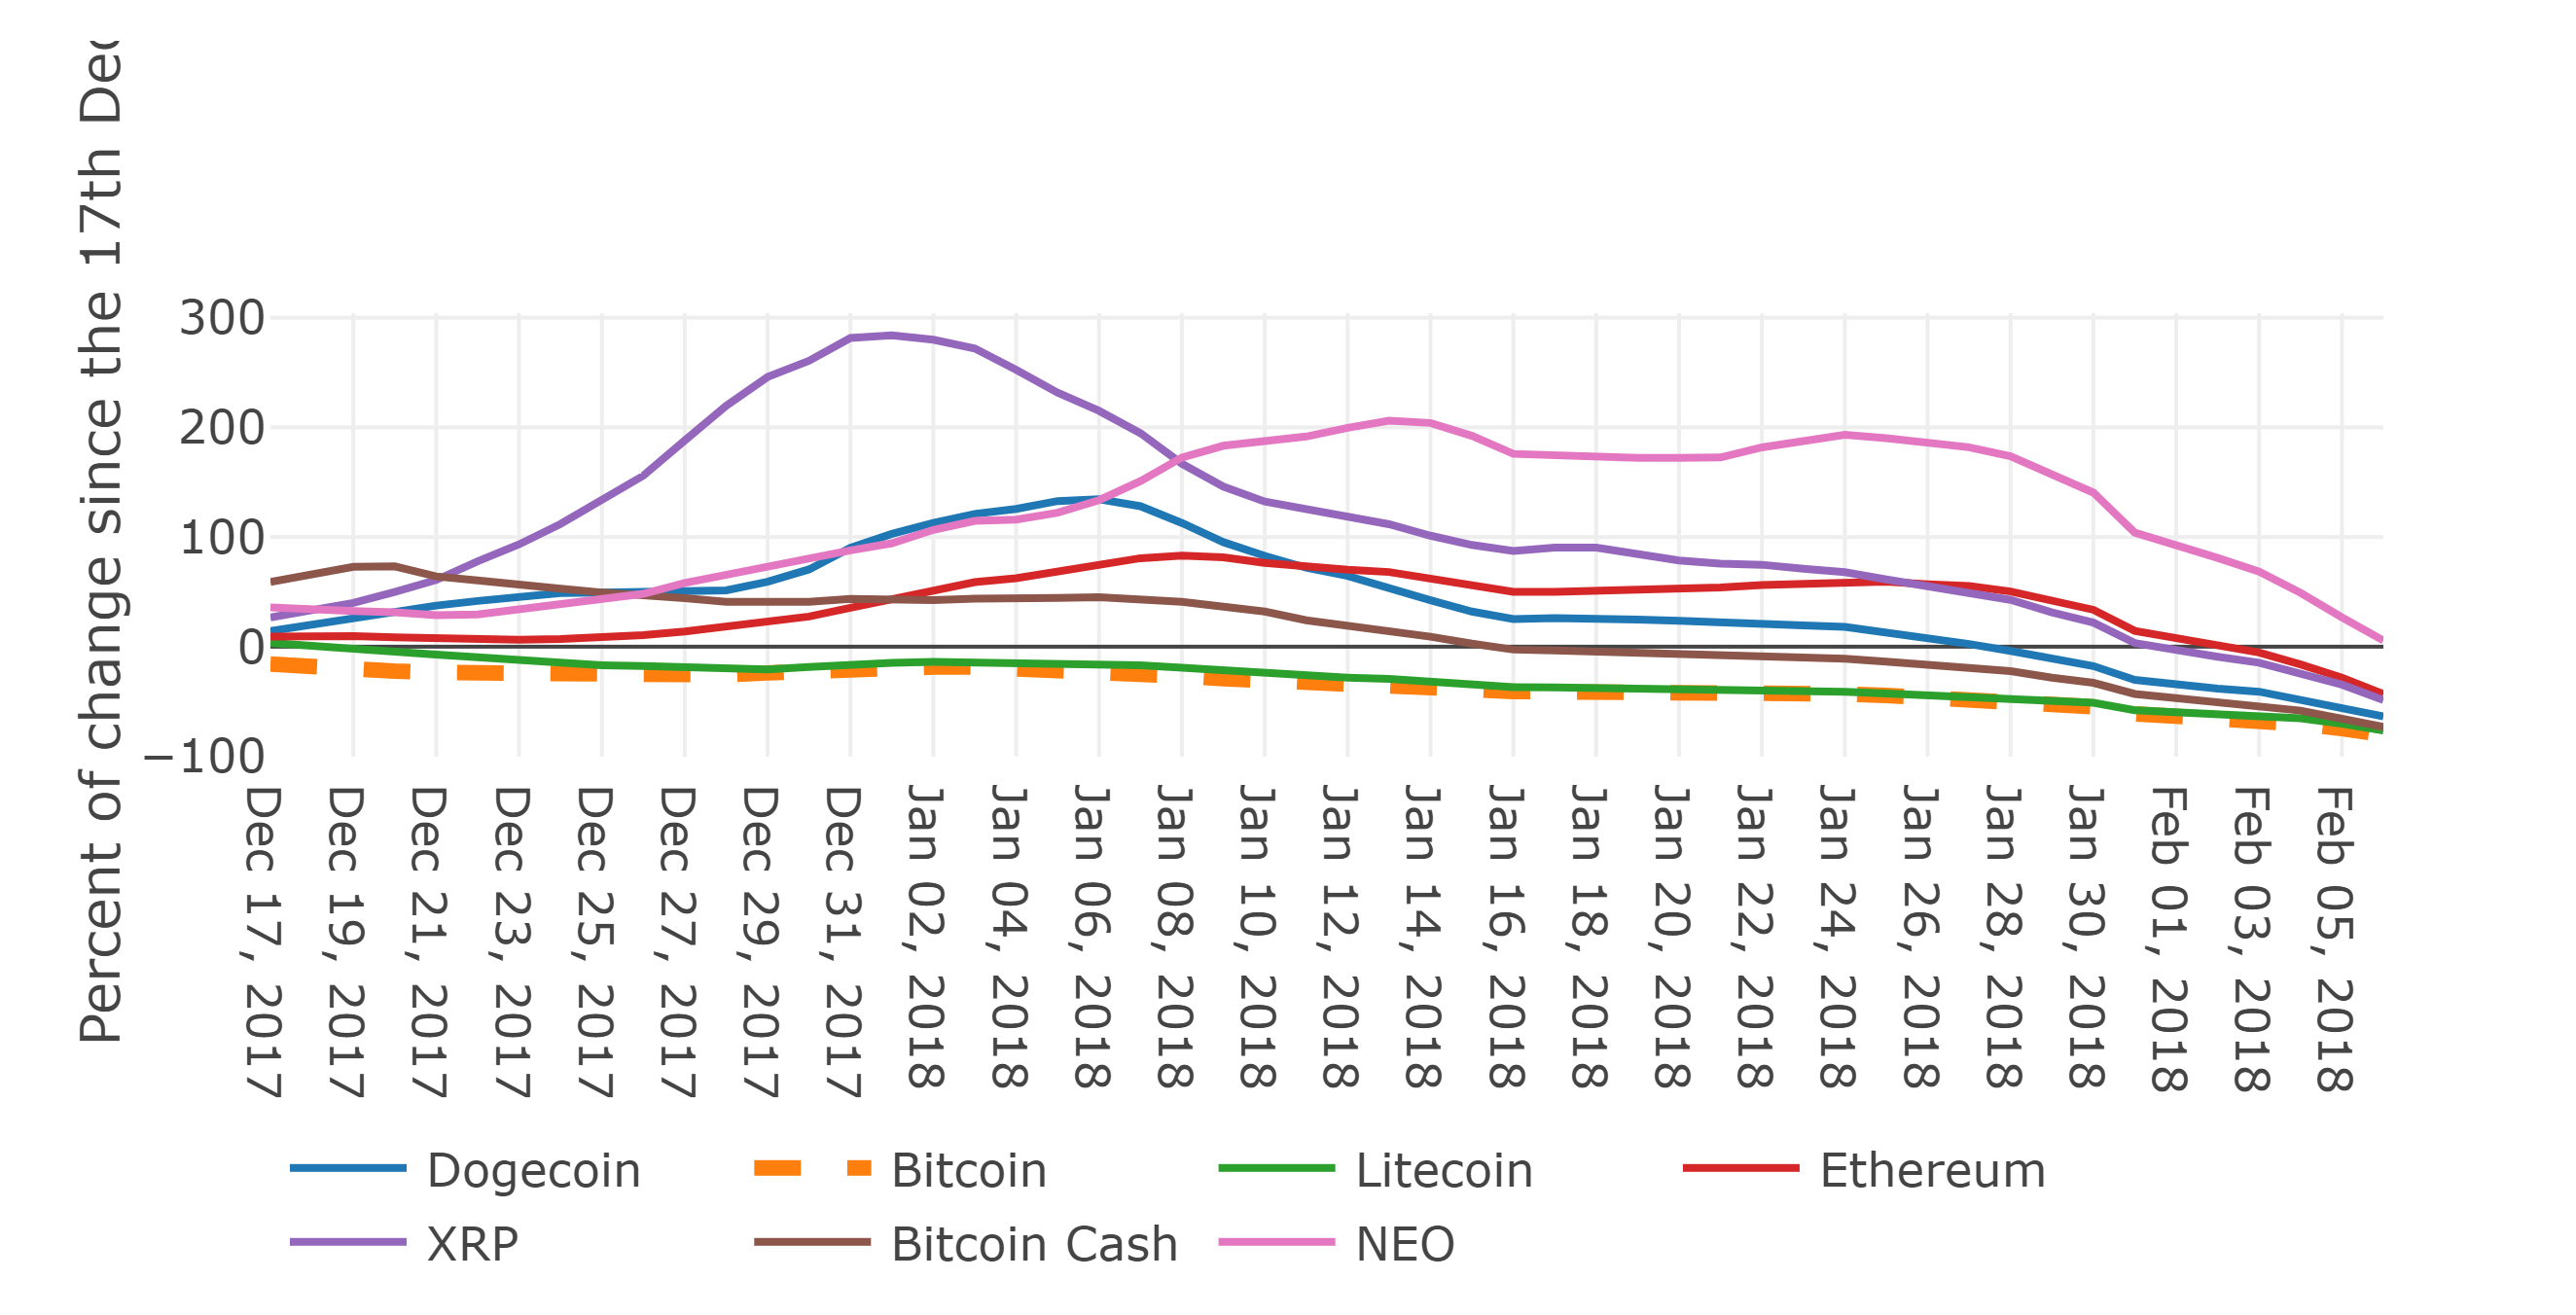
\includegraphics[width=\linewidth]{figures/diagram-20200618 (3).png}
    \caption[Change in value after the 2018 Bubble]{7 day rolling average over change in percent in comparison to the 17th of December 2017.}
    \label{fig:bubble2017}
\end{figure*}

After Bitcoin stabilized again, it more or less stayed constant in value, while the others depreciated more or less. When we look at the latest bubble, the bubble in 2018, we can see that the situation has changed. 



\autoref{fig:bubble2017} shows the value development for the biggest coins in 2018 in the time from the 17th December of 2017 (Bitcoins' peak) to 52 days later, the 6th February of 2018. It becomes apparent that most coins still hugely depreciate, but this time, Bitcoin is the biggest loser. Bitcoin reaches a low of \mbox{-80\%} at the opening of the markets on the 6th of February, most other coins have only lost between -44\% (Ethereum, XRP), and -75\%(Litecoin, Bitcoin Cash), with DogeCoin sitting in between with -63\%. As Litecoin and Bitcoin Cash can be considered as relatively close to Bitcoin, this is somewhat expected. 
There is one clear winner, however: NEO. On the 6th of February NEO managed to even gain 5\% of value since the 17th December, in a period where nearly all other currencies lost. 

\begin{table*}
\centering
\resizebox{\textwidth}{!}{%
\begin{tabular}{@{}l|c|llll@{}}
\toprule
Currency        & Market Entry & 2017 Value           & 2018 Value         & 2019 Value         & Value now              \\ \midrule
Bitcoin         & Jan 2009     & \$     2,577.77     & \$     2,590.92   & \$     7,826.90   & \$     8,788.73     \\
Ethereum        & Jul 2015     & \$        243.01    & \$        245.56  & \$        173.96  & \$       195.41 \\
Tether          & Feb 2015     & \$             1.00 & \$           1.00 & \$           1.00 & \$       1.00    \\
XRP             & Aug 2013     & \$             0.19 & \$           0.19 & \$           0.31 & \$           0.20   \\
Bitcoin Cash    & Jul 2017     & -                    & \$      540.16    & \$      272.64    & \$      249.06     \\
Bitcoin SV      & Nov 2018     & -                    & -                  & \$         93.42  & \$      195.00    \\
Litecoin        & Oct 2011     & \$           42.22  & \$         42.32  & \$         61.88  & \$         46.09   \\
Binance Coin    & Jul 2017     &  -                   & \$           1.53 & \$         19.48  & \$         16.66   \\
EOS             & Jul 2017     &  -                    & \$           1.42 & \$           3.66 & \$           2.75  \\
Cardano         & Oct 2017     & - & \$           0.03 & \$           0.05 & \$           0.05  \\
Crypto.com Coin & Dec 2018     & -                    & -                  & \$           0.04 & \$           0.05  \\
Tezos           & Sep 2017     &  -                   & \$           2.18 & \$           1.04 & \$           2.49   \\
Chainlink       & Sep 2017     &  -                    & \$           0.24 & \$           1.76 & \$           3.64 \\
Stellar         & Aug 2017     &  -                     & \$           0.02 & \$           0.08 & \$           0.06  \\
Monero          & May 2014     & \$           44.64  & \$         45.00  & \$         62.10  & \$         63.25    \\
UNUS SED LEO    & May 2019     & -                    & -                  &  -                     & \$           1.01   \\
Tron            & Sep 2017     & - & \$           0.00 & \$           0.02 & \$           0.02   \\
Huobi Token     & Feb 2018     & -                    & -                  & \$           2.98 & \$           3.91   \\
Neo             & Sep 2016     & \$             6.79 & \$           6.89 & \$           9.39 & \$         10.15    \\
 Coin        & Oct 2018     & -                    & -                  & \$           1.00 & \$           1.00  \\ \bottomrule
\end{tabular}%
}
\caption{The current top 20 cryptocurrencies. The values are in  and are the median over the year.}
\label{tab:my-table4}
\end{table*}

At the very beginning, other currencies also started to rise, when Bitcoin was already falling: Ethereum had doubled in value around the 9th of January, a time where DogeCoin too rose to around 120\%. The biggest rise however saw XRP: It was at its peak around new years nearly three times as much worth as roughly one month ago.

When looking at the difference of the coins which at least temporarily continued to rise, it becomes clear that they are all late entrant cryptocurrencies and have improved in different aspects. 

As an example, Ethereum has so-called smart contracts, which act like programs in the blockchain, which activate when certain requirements are met. This extends Ethereum to not only simple financial transactions but allows a wide variety of other functionality. Furthermore, it also used its own blockchain and used Ether, its own token, to power these before mentioned smart contracts and its decentralized marketplace\citep{ethereum}.

XRP, also sometimes called Ripple, on the other hand, saw one of Bitcoins' biggest problems, a long waiting period for financial transactions to be confirmed, and improved on that aspect. If in the Bitcoin ecosystem someone wants to send Bitcoins to someone else, for example at a store, no one wants to wait 30 minutes or more until the transaction has been confirmed a few times by the blockchain. However, this can only be avoided by paying a larger transaction fee, which can quickly cost a lot of money. Ripple was created to fix this and allow quick transaction (in the timeframe of seconds per transaction) very cheaply\citep{xrp}.

NEO took on the idea of Ethereum, by focusing on an efficient approach to deploy and also scale smart contracts on the own blockchain, with its long term vision of issuing and managing digital assets through the NEO blockchain\citep{neo}.

When looking at \autoref{fig:dominance} on the second page again, we can see that this time has had a big impact on Bitcoins' market share. It went from about 80\% in the first quarter of 2017 to 34\% around early 2018. Ethereums share increased to nearly 30\%, and XRPs to roughly 10\% before the bubble burst. After the bubble, these numbers have fallen again, but Bitcoin did not manage to regain the leadership role it had before. Ethereum is now down to 10\% and XRP to 3\%, but the percentage of other cryptocurrencies rose and rose since then. In total, the other currencies now make up for around 10\% of the total market share. And these are in many cases, even later entrants than Ethereum or Ripple.


\subsection{Bursting of the 2018 Bubble in the long run}
When we look we look at the time after the Bubble had burst, we can see the effect it, in the long run, had: pretty much none. 

The prices at first rose slowly in 2017 and then began to race quickly to the top at the end of the year. Thus lead to a median value of Bitcoin of \$2,577.77. When we look at the median value in 2018, which was \$2,590.92, we see that the difference is a mere \$13.15. 

Other coins experienced the same: Ethereum had in 2017 a median value of \$243.01  and in 2018 a value of \$245.56---a small difference of about \$2. Monero: up from \$44.64  to \$45.00  in the next year. 

It can be seen that while Bubbles lead to huge price differences in a relatively short time frame (the bubble in 2017--2018 lasted around 4 months, with 2 months rising quickly and 2 months falling seemingly endlessly), in the end, they do not have too much impact on the price in the long run. 

On the other hand, this does not mean that everyone will profit from bubbles at the end of the day. When we look at the median value of 2019 and the median value until now, we can see that while Bitcoin rose quite drastically again, others did not perform the same: Ethereum fell in 2019 to around \$173 for most of the time and only managed to rise again as of lately. 


Monero rose in 2019 compared to 2018 and stayed relatively stable at around \$62  until now. Like Bitcoin, Monero did not fall when we just look at the median values but did not catch on to the trend of rising again. Bitcoin Cash is still on its downfall to this very date.

When looking at coins which were created after the bubble, like Bitcoin SV, Crypto.com Coin or furthermore the Huobi Token, we can see that they are all on a strong upward trend, with the exception to the USD-Coin, which is bound to the U.S. Dollar and therefore will not experience any price fluctuations. Bitcoin SV rose from the median value in 2019 to the median value until now roughly 95\%, Crypo.com, went up 25\% in its price, and Huobi 31\%. It should be noted that the last ones accomplished a price difference of \$0.01  and \$0.93  respectively, which certainly is not a huge sum---yet take into account that we are looking at the top 20 currencies with a correspondingly high market capitalization (Huobi is just shy of one billion U.S Dollar and Crypto.com has around \$2.3 billion  in market capitalization).  



\section{Discussion}

\begin{figure*}[ht]
  \centering
  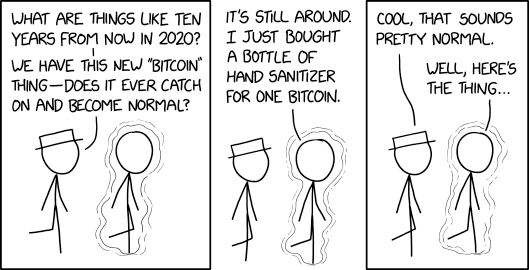
\includegraphics[width=\linewidth]{figures/2010_and_2020.png}
  \caption[xkcd comic]{Source: \cite{xkcd}. Hover text: ``2030: `I just bought a house for one Bitcoin. No, It is the equivalent of a dollar. Houses are often transferred for a nominal fee because the buyer is taking responsibility for containing the holo-banshees in the attic.'"}
  \label{xkcd}
\end{figure*} 

To sum up: Cryptocurrencies are a highly volatile market. The median values have been quite consistent in the last 3 years for the top 20 cryptocurrencies, with a small trend in rising again. However, when looking at the changes in price from day to day, one can see that they still fluctuate very strongly up and down. 

Being an unregulated market, cryptocurrencies often attract fraudulent behavior. This can be evidenced either by market manipulation, like the Bitcoin bubble in 2013, or exit scams, like what had happened with the cryptocurrency exchange WEX. Events like the latter often lead to huge losses for people, who had put their faith into the system. When Mt.Gox went offline, it took seven percent of all Bitcoins with it---something which can be catastrophic, when the total amount of coins is actually limited.

Whether someone profits immensely or loses most of his investment also depends on the price when he bought the currency. If someone had bought Bitcoins during the beginning of the bubble, he would have had stellar profits---but only if he also sold at the highest point, which is impossible to know before without insider information. If someone bought quickly after the initial fall, betting on quickly rising prices again, he would not have recovered his investment to this date.  

When asking the question of whether cryptocurrencies are going to stay or are going to be a thing of the past, one will notice that there is no exact answer. Only time will tell, but there are a few indicators that might lead to an abandonment at a later point in time. 

Bitcoin for example has a few major problems. For one, Bitcoins transaction management is too slow for an actual application in a real-world Point of Sale. Without paying high transaction fees, the time until a transaction is confirmed is usually around 60 mins. It might be a solution for an e-commerce application, but It is simply unacceptably high for shopping at a local store. Transactions in real-time would require exorbitant high fees and only a few confirmations required, leading to a higher risk of fraud. Litecoin tried to improve on this early on but failed to find its groundbreaking success yet. XRP was subsequently founded to offer actual support for this scenario by offering quick transaction times around five to seven seconds, but also did not replace Bitcoins leadership in market dominance.

Furthermore, many have pointed out the catastrophic consequences of Bitcoin mining for the environment. A recent study pointed out that the annual carbon emissions range from 22.0 to 22.9 Mt CO, which sits between the levels produced by actual nations, namely of Jordan and Sri Lanka \citep{carbon}. There have been a few cryptocurrencies developed with the goal of being climate-friendly and moreover sustainable, but they never did catch on. Burst Coin uses a proof of stake algorithm for mining, making it more efficient to mine on a consumer PC. CoinMarketCap ranks it at the 413th place, and it is mostly abandoned nowadays. Nano seems to be another option, ranked at the 55th place. It is mostly energy-less by not using the conventional approach to mining. But then again, It is still only the 55th place, meaning that 54 less environmentally friendly currency are currently preferred.

The biggest problem of Bitcoin as an actual currency and not just an object of speculation is its massive price volatility. It simply is unusable, when the value of a Bitcoin changes from day to day. On the 19th of June 2020, the markets opened with a value of \$9,410.29. A day before they had opened with a value of \$9.481,57, a difference of \$71  in a day. At this point, it becomes impossible to calculate a price in Bitcoin, because you cannot know what tomorrow's price will be. Currencies like Tether and  Coin have fixed this by valuing a coin at \$1, but then again suffer the same before mentioned problems as Bitcoin. For example, Tether's transaction time depends on the chosen network and is something between six and sixty minutes. 

These concerns have been expressed by others too, such as the Bank for International Settlements\citep{hype}. Bitcoin has been described as an economic bubble by at least three Nobel Memorial Prize in Economic Sciences laureates \citep{robert,stiglitz,thaler} and many other noted economists \citep{kearns,guardian,krugman}. 

Of course, there are more cryptocurrencies than Bitcoin today. But Bitcoin is still the leader in the market and other cryptocurrencies did not yet manage to throw it off its thrown completely. The answer to the question if cryptocurrencies are going to stay or are going to be a thing of the past is defined by the acceptance of them. If people start to use cryptocurrencies in their everyday business, then they are here to stay. But if they continue to be an object of speculation, with prices changing every day, then they will not be from any value as a currency. 

Because clearly, no one wants to be that guy who paid 10,000 Bitcoins for a pizza \citep{pizzaguy}. 

\newpage

\printbibliography[title={Bibliography}] % Print the bibliography, section title in curly brackets
\pagebreak
\listoffigures

\end{document}
